\section{Long exact homology sequence, Excision, and Genealogy}
WARNING: I've probably messed up typing some indices. Hopefully not.
\subsection{5-lemma}
Suppose you have two exact sequences of abelian groups.
\begin{equation*}
\xymatrix{A_4\ar[r]^d\ar[d]^{f_4} & A_3\ar[r]^d\ar[d]^{f_3} & A_2\ar[r]^d\ar[d]^{f_2} & A_1\ar[r]^r\ar[d]^{f_1} & A_0\ar[d]^{f_0}\\
B_4\ar[r]^d & B_3\ar[r]^d & B_2\ar[r]^d & B_1\ar[r]^r & B_0}
\end{equation*}
When can we guarantee that $f_2$ is an isomorphism? We're going to diagram chase :-(. Just follow your nose.

Let $b_2\in B_2$. We want to show that there is something in $A_2$ that can be pushed forward to $b_2$, i.e., prove surjectivity of $f_2$. We can consider $db_2\in B_1$. Let's assume that $f_1$ is surjective. Then there's $a_1\in A_1$ such that $f_1(a_1)=db_2$. What is $da_1$? Well, $f_0(da_1)=d(f_1(a_1))=d(db)=0$. So we want $f_0$ to be injective. Then $da_1$ is zero, so by exactness of the top sequence, there is some $a_2\in A_2$ such that $da_2=a_1$. What is $f_2(a_2)$? What is $d(f_2(a_2))$? By commutativity, $d(f_2(a_2))=f_1(d(a_2))=f_1(a_1)=db_2$. Let's consider $b_2-f_2(a_2)$. This maps to zero under $d$. So by exactness, there is $b_3\in B_3$ such that $d(b_3)=b_2-f_2(a_2)$. If we assume that $f_3$ is surjective, then there is $a_3\in A_3$ such that $f_3(a_3)=b_3$. But now, $d(a_3)\in A_2$, and $f_2(d(a_3))=d(f_3(a_3))=b_2-f_2(a_2)$. But this means that $b_2=f(a_2+d(a_3))$, which guarantees surjectivity of $f_2$. This means that if $f_1$ is surjective, $f_0$ is injective, and $f_3$ is surjective, then $f_2$ is surjective.

A similar dual process says that $f_2$ is injective if $f_1$ is injective, $f_3$ is injective, and $f_4$ is surjective. If all of these conditions are satisfied, then $f_2$ is an isomorphism. This is the content of the five-lemma.
\subsection{Relative homology}
I guess I didn't really define this. Suppose you have a pair of spaces $(X,A)$. Then you have an sexseq of chain complexes $0\to S_\ast(A)\to S_\ast(X)\to S_\ast(X,A)\to 0$. 
\begin{definition}
The relative homology of the pair $ H_\ast(X,A):= H(S_\ast(X,A))$.
\end{definition}
\begin{example}
$ H_\ast(X,\emptyset)= H_\ast(X)$ because $S_\ast(\emptyset)=0$. Another case is $ H_\ast(X,X)=0$ because $S_\ast(X,X)=S_\ast(X)/S_\ast(X)=0$.
\end{example}
\subsection{General study of homologies of sexseqs of chain complexes}
Suppose I have three chain complexes $A_\bullet\to B_\bullet\to C_\bullet$. By the way, this is an important announcement. Henceforth, differentials in chain complexes will be denoted $d$, no longer $\partial$. For some reason. (It's so much easier for typing as well.) Assume that this is an exact sequence of chain complexes.

Is $ H_\ast(A)\to H_\ast(B)\to H_\ast(C)$ exact? Let's push this a little further. Suppose I have a sexseq $0\to A_\bullet\to B_\bullet\to C_\bullet\to 0$. We can ask the same question as before. Let's write this out more explicitly.
\begin{equation*}
\xymatrix{0\ar[r] & A_{n+1}\ar[r]^f\ar[d]^d & B_{n+1}\ar[r]^g\ar[d]^d & C_{n+1}\ar[r]\ar[d]^d & 0\\
0\ar[r] & A_n\ar[r]^f\ar[d]^d & B_n\ar[r]^g\ar[d]^d & C_n\ar[r]\ar[d]^d & 0\\
0\ar[r] & A_{n-1}\ar[r]^f & B_{n-1}\ar[r]^g & C_{n-1}\ar[r] & 0}
\end{equation*}
Let $[b]\in H_n(B)$ such that $g([b])=0$. It's determined by some $b\in B_n$ such that $d(b)=0$. If $g([b])=0$, then there is some $\overline{c}\in C_{n+1}$ such that $d\overline{c}=gb$. Now, $g$ is surjective, so there is some $\overline{b}\in B_{n+1}$ such that $g(\overline{b})=\overline{c}$. Then we can consider $d\overline{b}\in B_n$, and $g(d(\overline{b}))=d(\overline{c})\in C_n$. What is $b-d\overline{b}$? This maps to zero in $C_n$, so by exactness there is some $a\in A_n$ such that $f(a)=b-d\overline{b}$. Is $a$ a cycle? Well, $f(da)=d(fa)=d(b-d\overline{b})=db-d^2\overline{b}=db$, but we assumed that $db=0$, so $f(da)=0$. This means that $da$ is zero because $f$ is an injection by exactness. Therefore $a$ is a cycle. What is $[a]\in H_n(A)$? Well, $f([a])=[b-d\overline{b}]=[b]$ because $d\overline{b}$ is a cycle. Is the composite $ H_n(A)\to H_n(B)\to H_n(C)$ zero? Yes, because the composite factors through zero. This proves exactness of $ H_n(A)\to H_n(B)\to H_n(C)$.

\begin{theorem}[lexseq in homology]
Let $0\to A_\bullet\to B_\bullet\to C_\bullet\to 0$ be a sexseq of chain complexes. Then there is a natural homomorphism $\partial: H_n(C)\to H_{n-1}(A)$ such that there's lexseq:
\begin{equation*}
\xymatrix{ & & \ar[dll]^\partial\\
 H_n(A)\ar[r] & H_n(B)\ar[r] & H_n(C)\ar[dll]^\partial\\
 H_{n-1}(A)\ar[r] & H_{n-1}(B)\ar[r] & H_{n-1}(C)\ar[dll]^\partial\\
 & & &}
\end{equation*}
\end{theorem}
\begin{proof}
We'll construct $\partial$, and leave the rest as an exercise. We have our sexseq:
\begin{equation*}
\xymatrix{0\ar[r] & A_{n+1}\ar[r]^f\ar[d]^d & B_{n+1}\ar[r]^g\ar[d]^d & C_{n+1}\ar[r]\ar[d]^d & 0\\
0\ar[r] & A_n\ar[r]^f\ar[d]^d & B_n\ar[r]^g\ar[d]^d & C_n\ar[r]\ar[d]^d & 0\\
0\ar[r] & A_{n-1}\ar[r]^f & B_{n-1}\ar[r]^g & C_{n-1}\ar[r] & 0}
\end{equation*}
Let $c\in C_n$ such that $dc=0$. The map $g$ is surjective, so pick a $b\in B_n$ such that $g(b)=c$. Then consider $db\in B_{n-1}$. But $g(d(b))=0=d(g(b))=dc$. So by exactness, there is some $a\in A_{n-1}$ such that $f(a)=db$. How many choices are there of picking $a$? One, because $a$ is injective. We need to check that $a$ is a cycle. What is $d(a)$? Well, $d^2b=0$, so $da$ maps to $0$ under $f$. But because $f$ is injective, $da=0$, i.e., $a$ is a cycle. This means we can define $\partial[c]=[a]$.

To make sure that this is well-defined, let's make sure that this choice of homology class $a$ didn't depend on the $b$ that we chose. Pick some other $b^\prime$ such that $g(b^\prime)=c$. Then there is $a^\prime\in A_{n-1}$ such that $f(a^\prime)=db^\prime$. We want $a-a^\prime$ to be a boundary, so that $[a]=[a^\prime]$. We want $\overline{a}\in A_n$ such that $d\overline{a}=a-a^\prime$. Well, $g(b-b^\prime)=0$, so by exactness, there is $\overline{a}\in A_n$ such that $f(\overline{a})=b-b^\prime$. What is $d\overline{a}$? Well, $d\overline{a}=d(b-b^\prime)=db-db^\prime$. But $f(a-a^\prime)=b-b^\prime$, so because $f$ is injective, $d\overline{a}=a-a^\prime$, i.e., $[a]=[a^\prime]$. What else do I have to check? It's an exercise to check that $\partial$ as defined here is a homomorphism. Also, left as an exercise to check that this doesn't depend on $c\in[c]$, and that $\partial$ actually makes the exact sequence above exact.
\end{proof}
\subsection{Mathematical Genealogy}
I'm not typing in anything here. It's a rather big tree:
\begin{figure}[H]
\centering
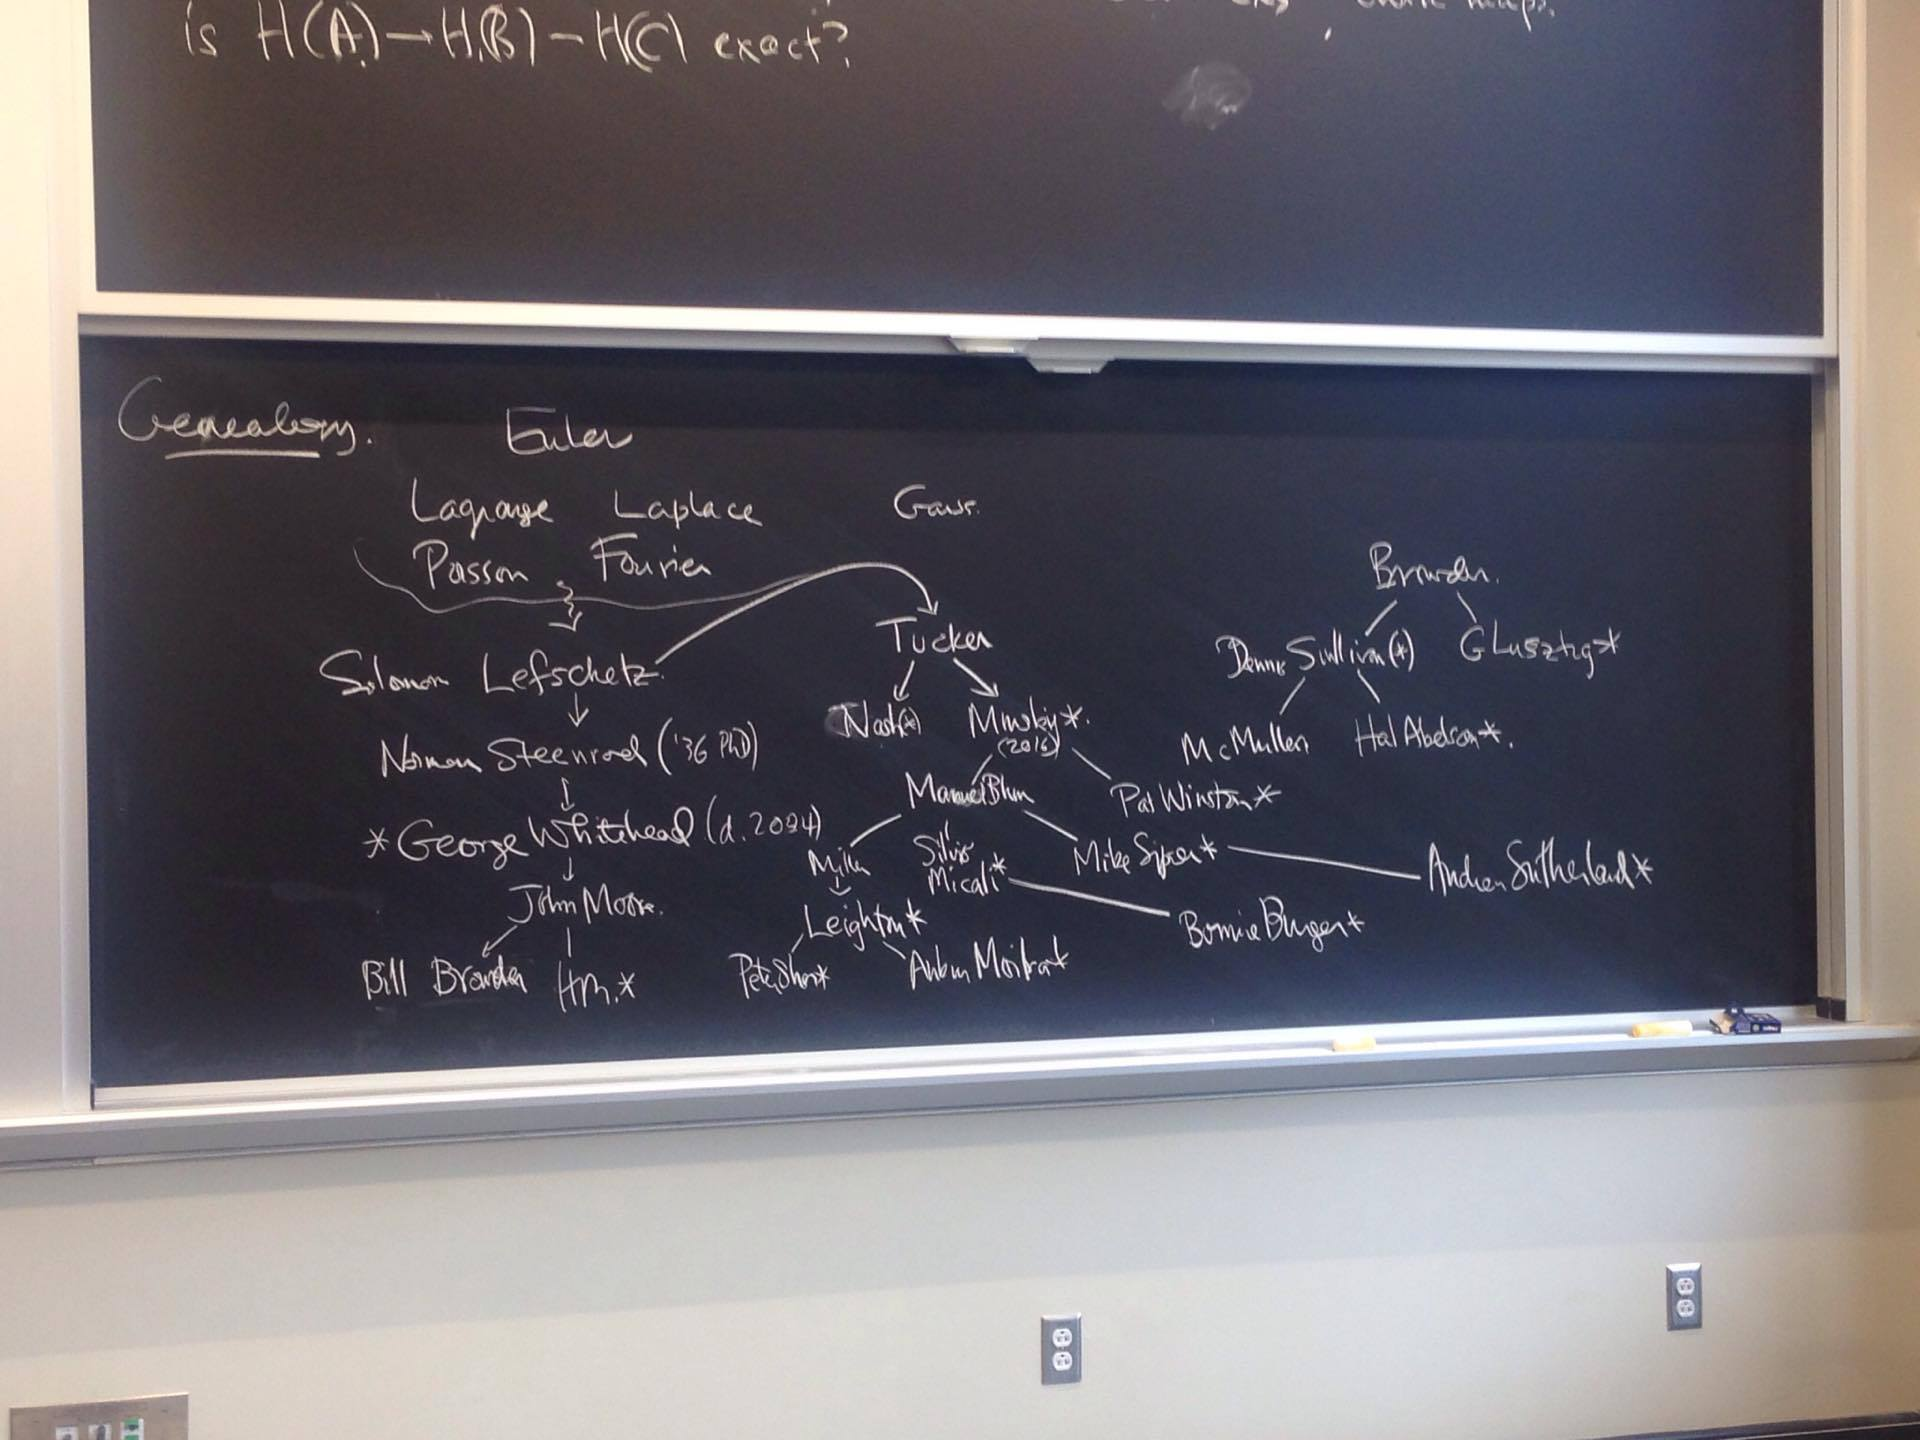
\includegraphics[width=\textwidth]{assets/math-family}
\caption{Mathematical genealogy, growing from Lefschetz, who was initially a chemist. The asterisks are meant to indicate that someone's at MIT.}
\end{figure}
